\chapter{Design sketches}\label{design-sketches}
I didn't use a tool, because the design is not standardized, and it's easier and faster drawing by hand then by a tool.

\todo{szebben lerajzolni vonalzóval!!!!! vagy megcsinálni az egészet egy tool-lal, mert ez így csúnya}
%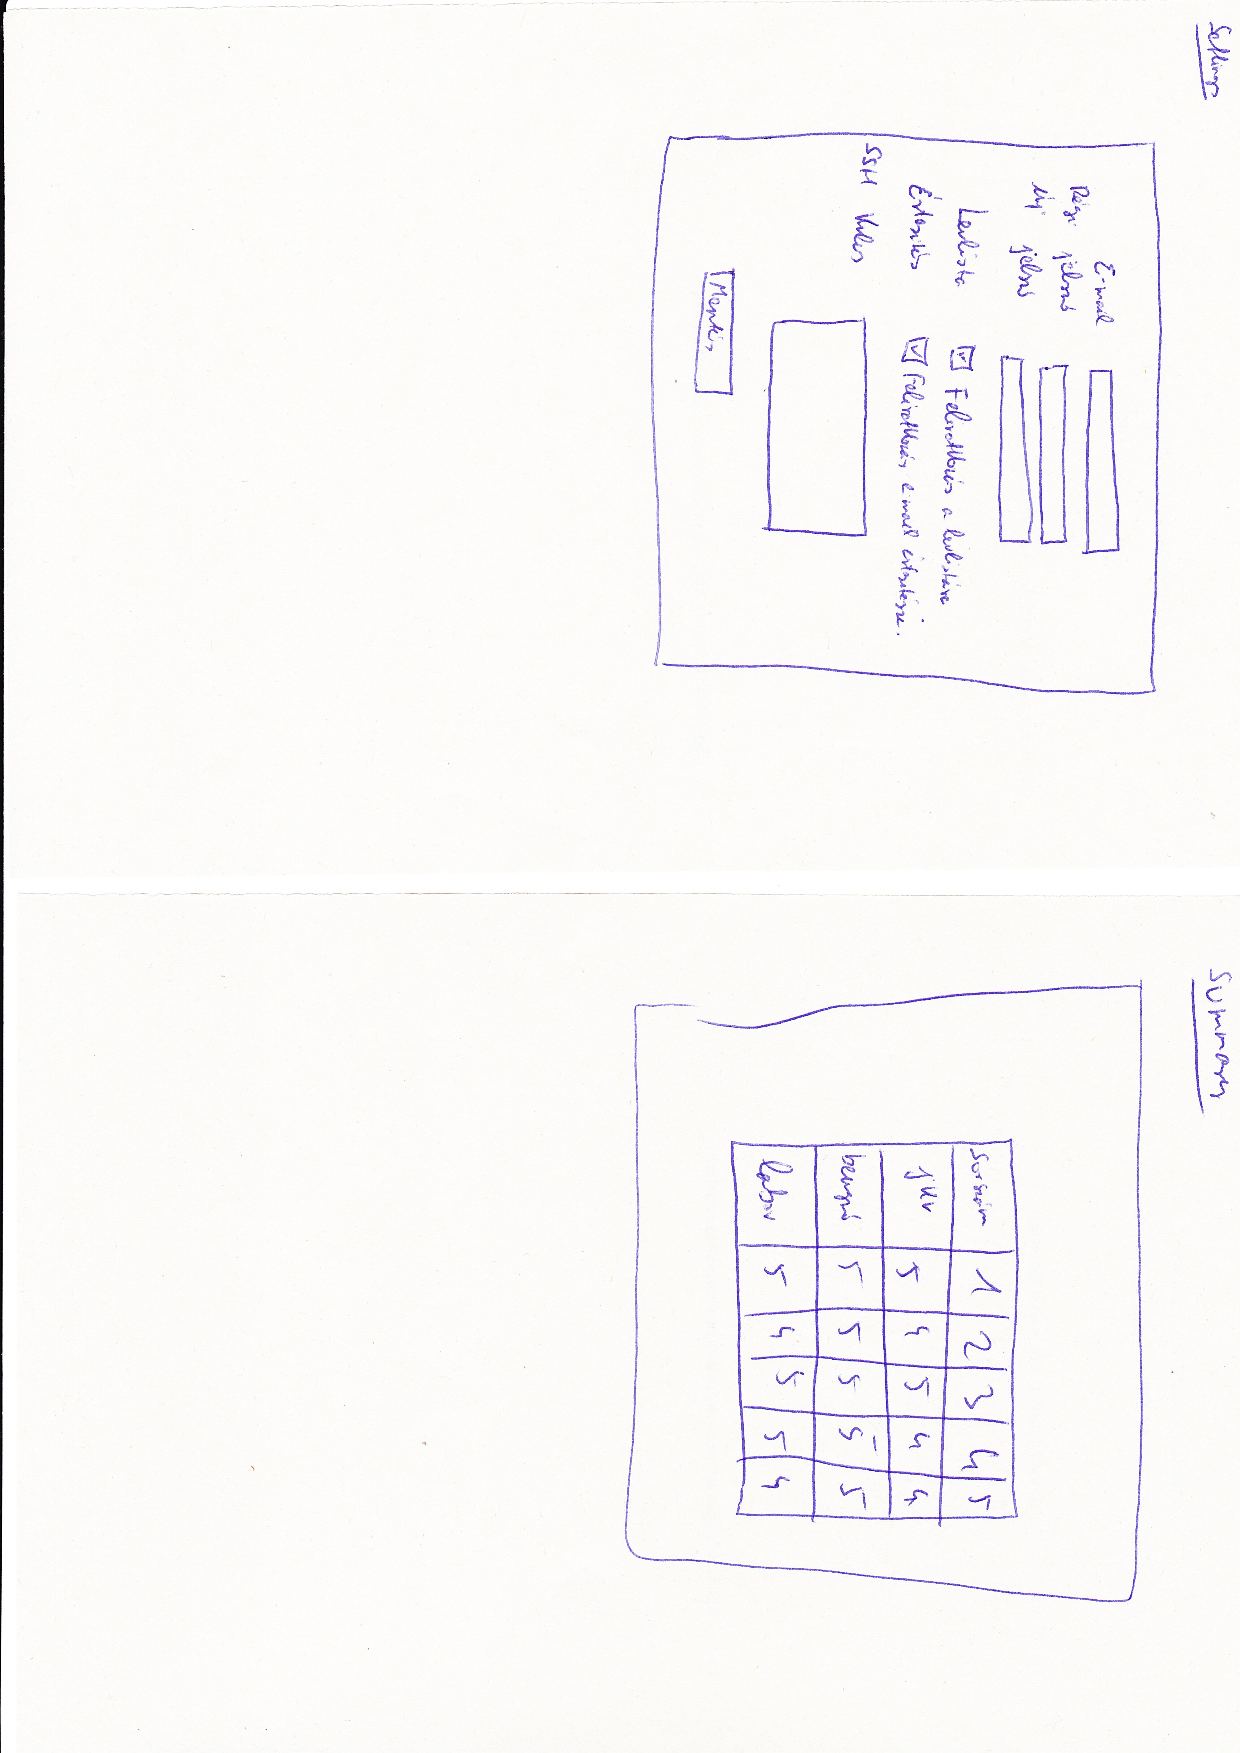
\includepdf[pages=-]{figures/sketches.pdf}
\begin{figure}[!ht]
	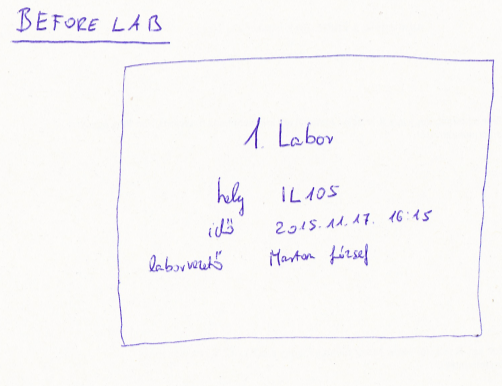
\includegraphics[width=\textwidth]{figures/sketch5.png}
	\caption{Laboratory page sketch, before lab}
	\label{fig:sketch5}
\end{figure}

\begin{figure}[!ht]
	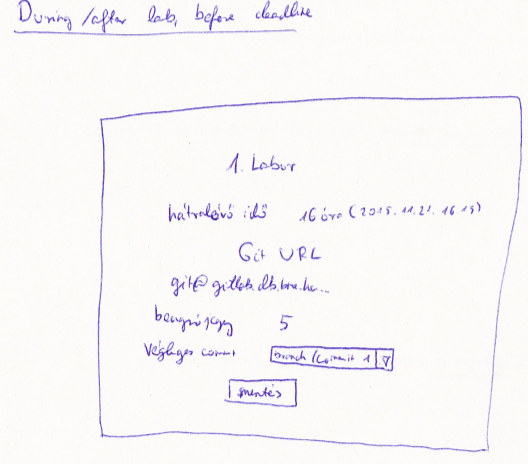
\includegraphics[width=\textwidth]{figures/sketch3.png}
	\caption{Laboratory page sketch, during/after lab, before deadline}
	\label{fig:sketch3}
\end{figure}

\begin{figure}[!ht]
	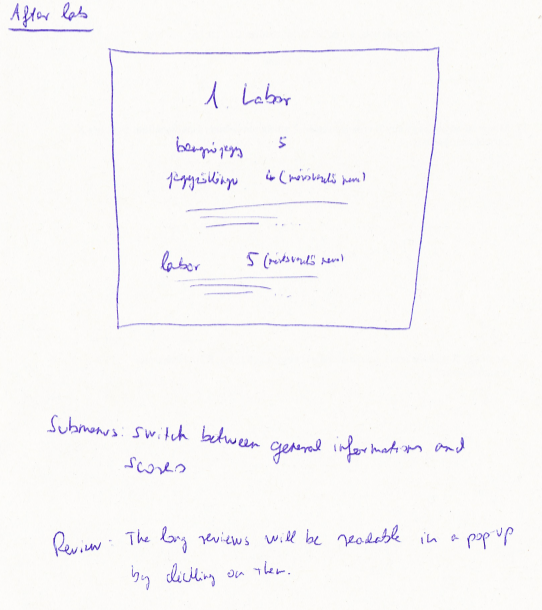
\includegraphics[width=\textwidth]{figures/sketch4.png}
	\caption{Laboratory page sketch, after lab}
	\label{fig:sketch4}
\end{figure}

\begin{figure}[!ht]
	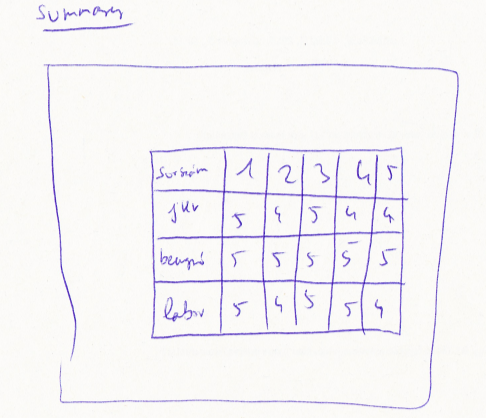
\includegraphics[width=\textwidth]{figures/sketch2.png}
	\caption{Summary page sketch}
	\label{fig:sketch2}
\end{figure}

\begin{figure}[!ht]
	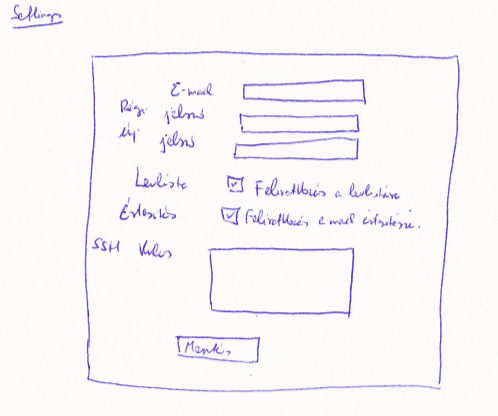
\includegraphics[width=\textwidth]{figures/sketch1.png}
	\caption{Settings page sketch}
	\label{fig:sketch1}
\end{figure}